\section{AMemGym 的三阶段框架}

\begin{importantbox}{框架结论}
本章的核心结论是：AMemGym 把长程对话记忆评测拆成三个相互衔接的阶段，先用结构化状态生成可控的用户事实变化，再让被测 agent 进入 on-policy interaction，最后在多个 checkpoint 注入 memory query 并用 diagnostic metrics 定位失败环节。这样，评测同时保留了真实交互中的上下文耦合、可追踪的 ground truth，以及面向优化的诊断信号。
\end{importantbox}

上一章已经说明，on-policy evaluation 的关键在于让 agent 的回复进入后续上下文。AMemGym 的框架设计正是围绕这个前提展开：如果要评估长期记忆，测试系统必须先知道“真实状态”如何随时间变化，再让 agent 在对话中亲自经历这些变化，最后检查它能否在需要时准确回忆和使用相关信息。视频在 00:07:06 之后给出的框架总览将这个过程概括为三阶段 pipeline：Structured Data Generation、On-Policy Interaction 和 Fine-grained Evaluation。图~\ref{fig:amemgym-framework-overview} 先给出这条主流程，后文再逐段解释每个阶段承担的评测功能。

\begin{figure}[H]
  \centering
  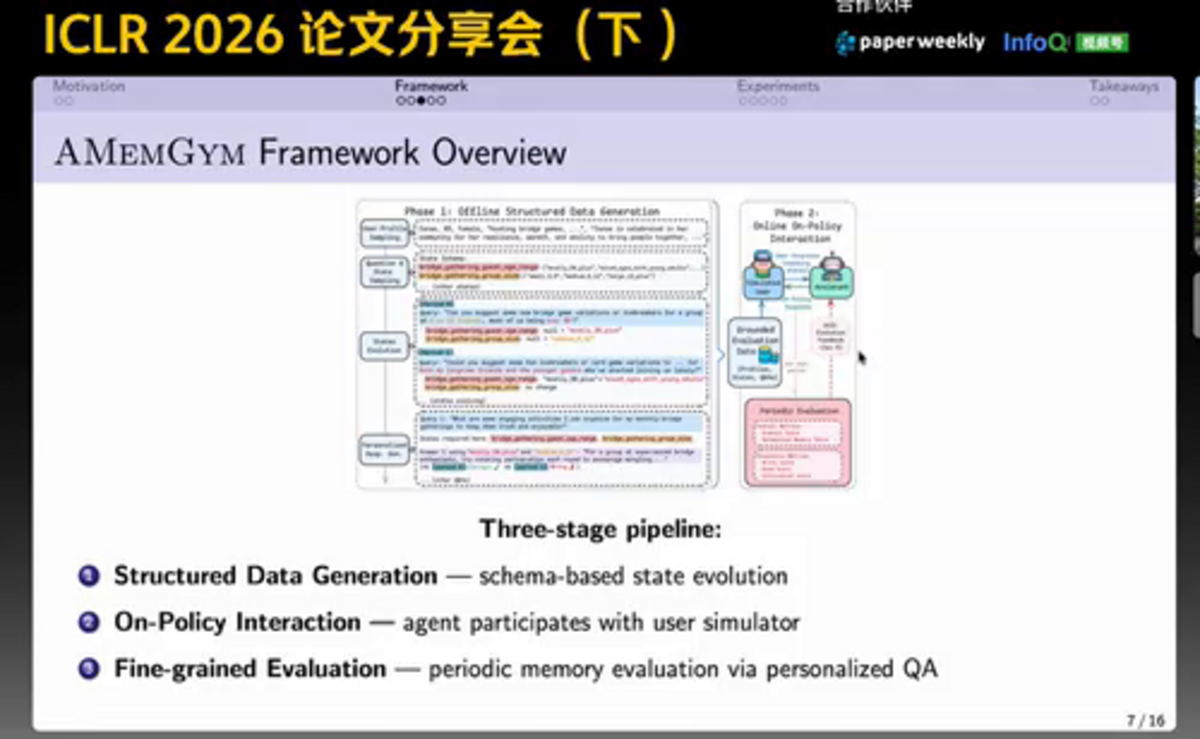
\includegraphics[width=0.82\linewidth,height=0.34\textheight,keepaspectratio]{figures/fig04_framework_overview.png}
  \caption[AMemGym 的三阶段框架总览]{AMemGym 的三阶段框架总览：结构化数据生成负责构造可控的状态演化，on-policy interaction 让 agent 与 user simulator 真实互动，细粒度评估在个性化问答中检查记忆能力。\protect\footnotemark}
  \label{fig:amemgym-framework-overview}
\end{figure}
\footnotetext{视频时间：00:07:06--00:08:00。}

\subsection{阶段一：用 schema-based state evolution 生成可控事实}

第一阶段解决的是“评测数据从哪里来”的问题。AMemGym 先定义 entity schema，也就是一套实体状态模板。一个实体可以理解为对话中需要长期追踪的对象，例如用户、活动、偏好、计划或关系；schema 则规定这个对象有哪些 attributes 和 relationships。用普通中文说，schema 像一张带字段说明的档案表：字段约定清楚后，系统才能知道后续状态变化到底改了哪一项。

视频中的例子是用户讨论 bridge gatherings。系统在不同 period 中更新 guest age range：Period 1 中是 \texttt{mostly\_50\_plus}，到 Period 3 时加入 \texttt{mixed\_ages\_with\_young\_adults}。这类变化在真实长期对话中很常见：用户的偏好会更新，计划会新增，旧信息会失效，关系也会发生调整。schema-based state evolution 的价值在于把这些变化显式记录下来，使每个时间点都能对应明确的 ground truth。图~\ref{fig:structured-data-generation} 展示了这种“先定结构、再更新状态”的生成方式。

\begin{figure}[H]
  \centering
  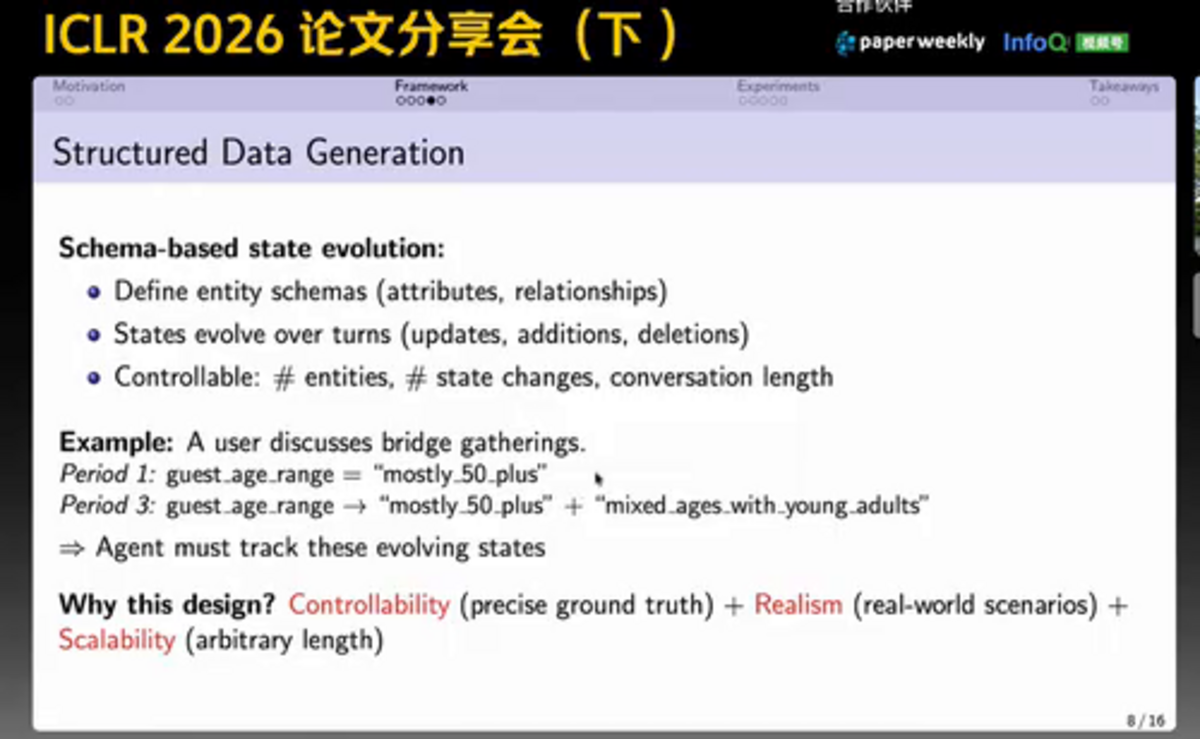
\includegraphics[width=0.82\linewidth,height=0.34\textheight,keepaspectratio]{figures/fig05_structured_data_generation.png}
  \caption[Structured Data Generation 阶段]{Structured Data Generation 阶段：先定义含 attributes 与 relationships 的 entity schema，再让 states 随 turns 发生 updates、additions 和 deletions。\protect\footnotemark}
  \label{fig:structured-data-generation}
\end{figure}
\footnotetext{视频时间：00:08:00--00:09:20。}

\begin{knowledgebox}{状态演化的直觉}
可以把 schema-based state evolution 类比为“带版本记录的用户档案”。普通聊天记录只告诉读者用户说过哪些句子；状态演化记录进一步说明这些句子背后的事实版本如何变化。对记忆评测而言，回答“当前状态是什么”通常比逐字复述某一句历史原文更关键。
\end{knowledgebox}

这一设计带来三个直接好处。第一是 controllability：评测者可以控制实体数量、状态变化次数和对话长度。第二是 realism：状态变化可以模拟真实对话中的信息流，例如偏好变更、计划推迟、人员范围扩大。第三是 scalability：当 schema 与演化规则确定后，对话可以扩展到更长范围，从而测试长程记忆在多轮累积后的表现。

\subsection{阶段二：让 agent 与 user simulator 形成 on-policy 轨迹}

第二阶段回答“这些状态如何进入对话”的问题。AMemGym 使用框架内的 user simulator，与被测 agent 进行多轮互动。user simulator 会按照前一阶段生成的状态演化，把相关事实逐步放进对话中；它的职责是形成可追踪的交互轨迹，开放式闲聊只占很小的教学价值。它像一次驾驶考试中的道路脚本：考官知道路线和突发情况，驾驶员仍然必须亲自操作，后续表现会受到前面每一步操作的影响。

在这个阶段，agent 的回复会成为对话历史的一部分。假设 agent 在某轮中误解了用户新加入的年龄范围，后续 user simulator 的追问与 agent 的上下文都会受到这个误解影响。AMemGym 因而获得的是 on-policy conversation trace，也就是被测 agent 亲自参与生成的交互轨迹。这个轨迹比读取固定剧本更贴近部署环境，因为长期记忆系统的写入、检索与使用都会在交互中留下痕迹。

\begin{warningbox}{模拟器边界}
这里容易出现一个误解：user simulator 并不等同于“真实用户样本越多越好”。它的核心职责是稳定传递可追踪的 state evolution，使每次评测都能追溯到明确 ground truth。如果模拟器只追求开放式闲聊，诊断阶段就会失去可控性，开发者很难判断失败来自写入、读取、使用，还是来自数据本身的漂移。
\end{warningbox}

\subsection{阶段三：在 checkpoint 中注入 memory query 并细粒度评估}

第三阶段处理“怎样判断 agent 记住了什么”的问题。AMemGym 会在多个预设 checkpoint 插入 personalized QA，也就是与当前用户状态相关的 memory query。checkpoint 可以理解为阶段性测验点；memory query 则是专门询问某个记忆点的问题。agent 需要从自己参与过的对话历史中回忆相关内容，并给出回答。

为了帮助读者把流程压缩成一个直观记号，本讲义引入下面的轻量表示；该记号只服务于讲义解释，视频没有把它作为论文公式给出：
\[
s_p \xrightarrow{\ \text{on-policy interaction}\ } q_p \xrightarrow{\ \text{evaluation}\ } r_p
\]
其中，\(s_p\) 表示第 \(p\) 个 period 后需要追踪的状态快照；\(q_p\) 表示在对应 checkpoint 注入的 memory query；\(r_p\) 表示 agent 对该 query 的回答。这个记号想表达的含义很简单：状态先通过互动进入轨迹，问题再从轨迹中抽查记忆，回答最后被评估。

评估层面包含两类信号。第一类是端到端的 QA accuracy，可作为 overall score。它告诉读者 agent 最终答对多少。第二类是更聚焦记忆能力的 score。视频说明，该类 score 会在 random baseline 与 perfect memory upper bound 之间做归一化，目的是把“会不会推理”和“有没有记住”尽量拆开观察。这里不加入额外公式，因为视频没有给出可直接复现的数学定义。

\subsection{diagnostic metrics：把失败拆成写、读、用}

AMemGym 更重要的贡献在于 diagnostic metrics。普通 overall score 只能告诉开发者“结果不好”；diagnostic metrics 进一步追问“坏在哪个环节”。视频把记忆失败拆成三个阶段：write failure、read failure 和 utilization failure。

write failure 指信息在写入记忆系统时已经丢失或写错。它像会议纪要一开始就漏记了关键决定，后面再怎么检索也找不到正确事实。read failure 指信息存在于记忆系统中，但检索、读取或定位失败。它像档案柜里确实有文件，索引却把人带到错误抽屉。utilization failure 指信息已经进入上下文，agent 仍然没有正确使用它。它像人拿到了正确资料，却在回答时忽略了资料的约束。

\begin{importantbox}{诊断指标的工程价值}
diagnostic metrics 的实际价值在于把“调参”变成“定位”。如果 write failure 高，开发者应检查哪些信息被写入、何时写入、是否过度压缩；如果 read failure 高，应检查检索策略、索引粒度和噪声；如果 utilization failure 高，应检查 agent 在生成答案时是否真正使用了已取回的记忆。
\end{importantbox}

这个拆解也解释了为什么 AMemGym 适合作为记忆系统优化工具。一个 agent 可能 QA accuracy 不高，但失败来源完全不同：有的系统写入太粗糙，有的系统检索太吵，有的系统拿到信息后仍然生成了不一致回答。只看总分会把这些机制差异压扁；加入 diagnostic metrics 后，开发者可以把优化目标对准具体环节。

\begin{warningbox}{术语校正边界}
字幕中出现的 \texttt{MMGM}、\texttt{i am gm} 按封面和图中标题统一写为 \texttt{AMemGym}；字幕中的 \texttt{diagnostic matrix} 按上下文校正为 \texttt{diagnostic metrics}。这些校正只处理明显 ASR 噪声。本章没有补写视频未给出的模型名单、精确数值或论文公式。
\end{warningbox}

\subsection{本章小结}

AMemGym 的三阶段框架可以概括为一条闭环：先用 schema-based state evolution 生成带 ground truth 的动态事实，再让 user simulator 把这些事实逐步注入 on-policy interaction，最后在 checkpoint 中用 memory query 和 diagnostic metrics 检查 agent 的长期记忆。三阶段分别承担可控性、真实性和可诊断性，合起来回应了前两章提出的问题：长程对话记忆评测需要保留 agent 自身回复对后续上下文的影响，也需要给开发者提供能够指导优化的失败分解。
